%%% Local Variables:
%%% mode: latex
%%% TeX-master: "<none>"
%%% End:

\label{sec:leaving}

An outgoing peer must to: (1) say $[\mathtt{goodbye}]$ to the splitter
and the neighbor peers (in this order), (2) relay any pending
(received but yet not sent) chunks, and (3) wait for a
$[\mathtt{goodbye}]$ from the splitter. In case of
timeout\footnote{All these messages are transmitted using a unreliable
  protocol.}, the leaving procedure is reset a number of times.

When a peer of the team receives a $[\mathtt{goodbye}]$, removes the
sender from its $\mathtt{forward}[]$ table. The splitter removes the
outgoing peer from the set of peers as soon as the
$[\mathtt{goodbye}]$ is received.

%Outgoing peers does not wait for a any reply from the neighbors to go.

\begin{comment}
\begin{figure*}
  %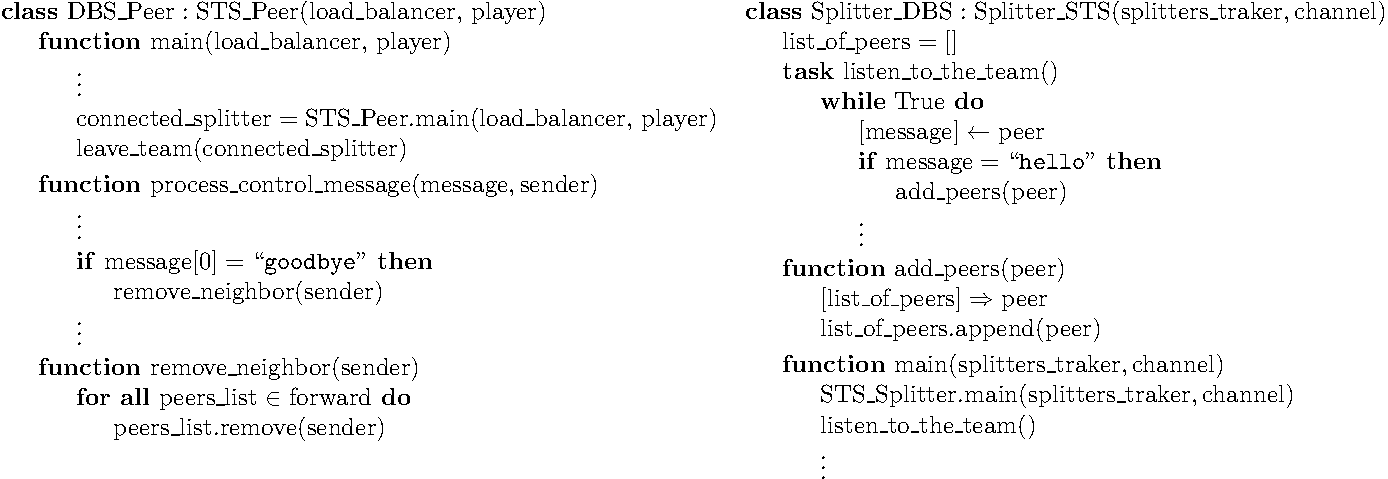
\includegraphics[width=0.55\textwidth]{leaving}
  \fig{400}{4cm}{leaving}
  \caption{Leaving a team.\label{fig:leaving}}
\end{figure*}

All these rules have been describen in Fig.~\ref{fig:leaving}.
\end{comment}

\begin{comment}
An outgoing peer $P_o$ (see Fig.~\ref{fig:leaving}) must to: (1) say
$[\mathtt{goodbye}]$ to $S$ and to $T^o$ (in this order), (2)
relay any pending (received but yet not sent) chunks, and (3) wait for
a $[\mathtt{goodbye}]$ from $S$, which performs $T = T \setminus
P_o$. In case of a timeout, $P_o$ resets the leaving procedure,
for a maximum number of times.

When a $P_k$ receives a $[\mathtt{goodbye}]$ from $P_o$, $P_k$
removes $P_o$ from its neighbors set, by running $T^k = T^k
\setminus P_o$.
\end{comment}
